\subsection{Estimación de los requisitos del equipo}
\clearpage
\thispagestyle{empty}

\addtolength{\oddsidemargin}{-55pt}
\addtolength{\evensidemargin}{-70pt}
\addtolength{\topmargin}{-90pt}

\begin{figure}[!h]
  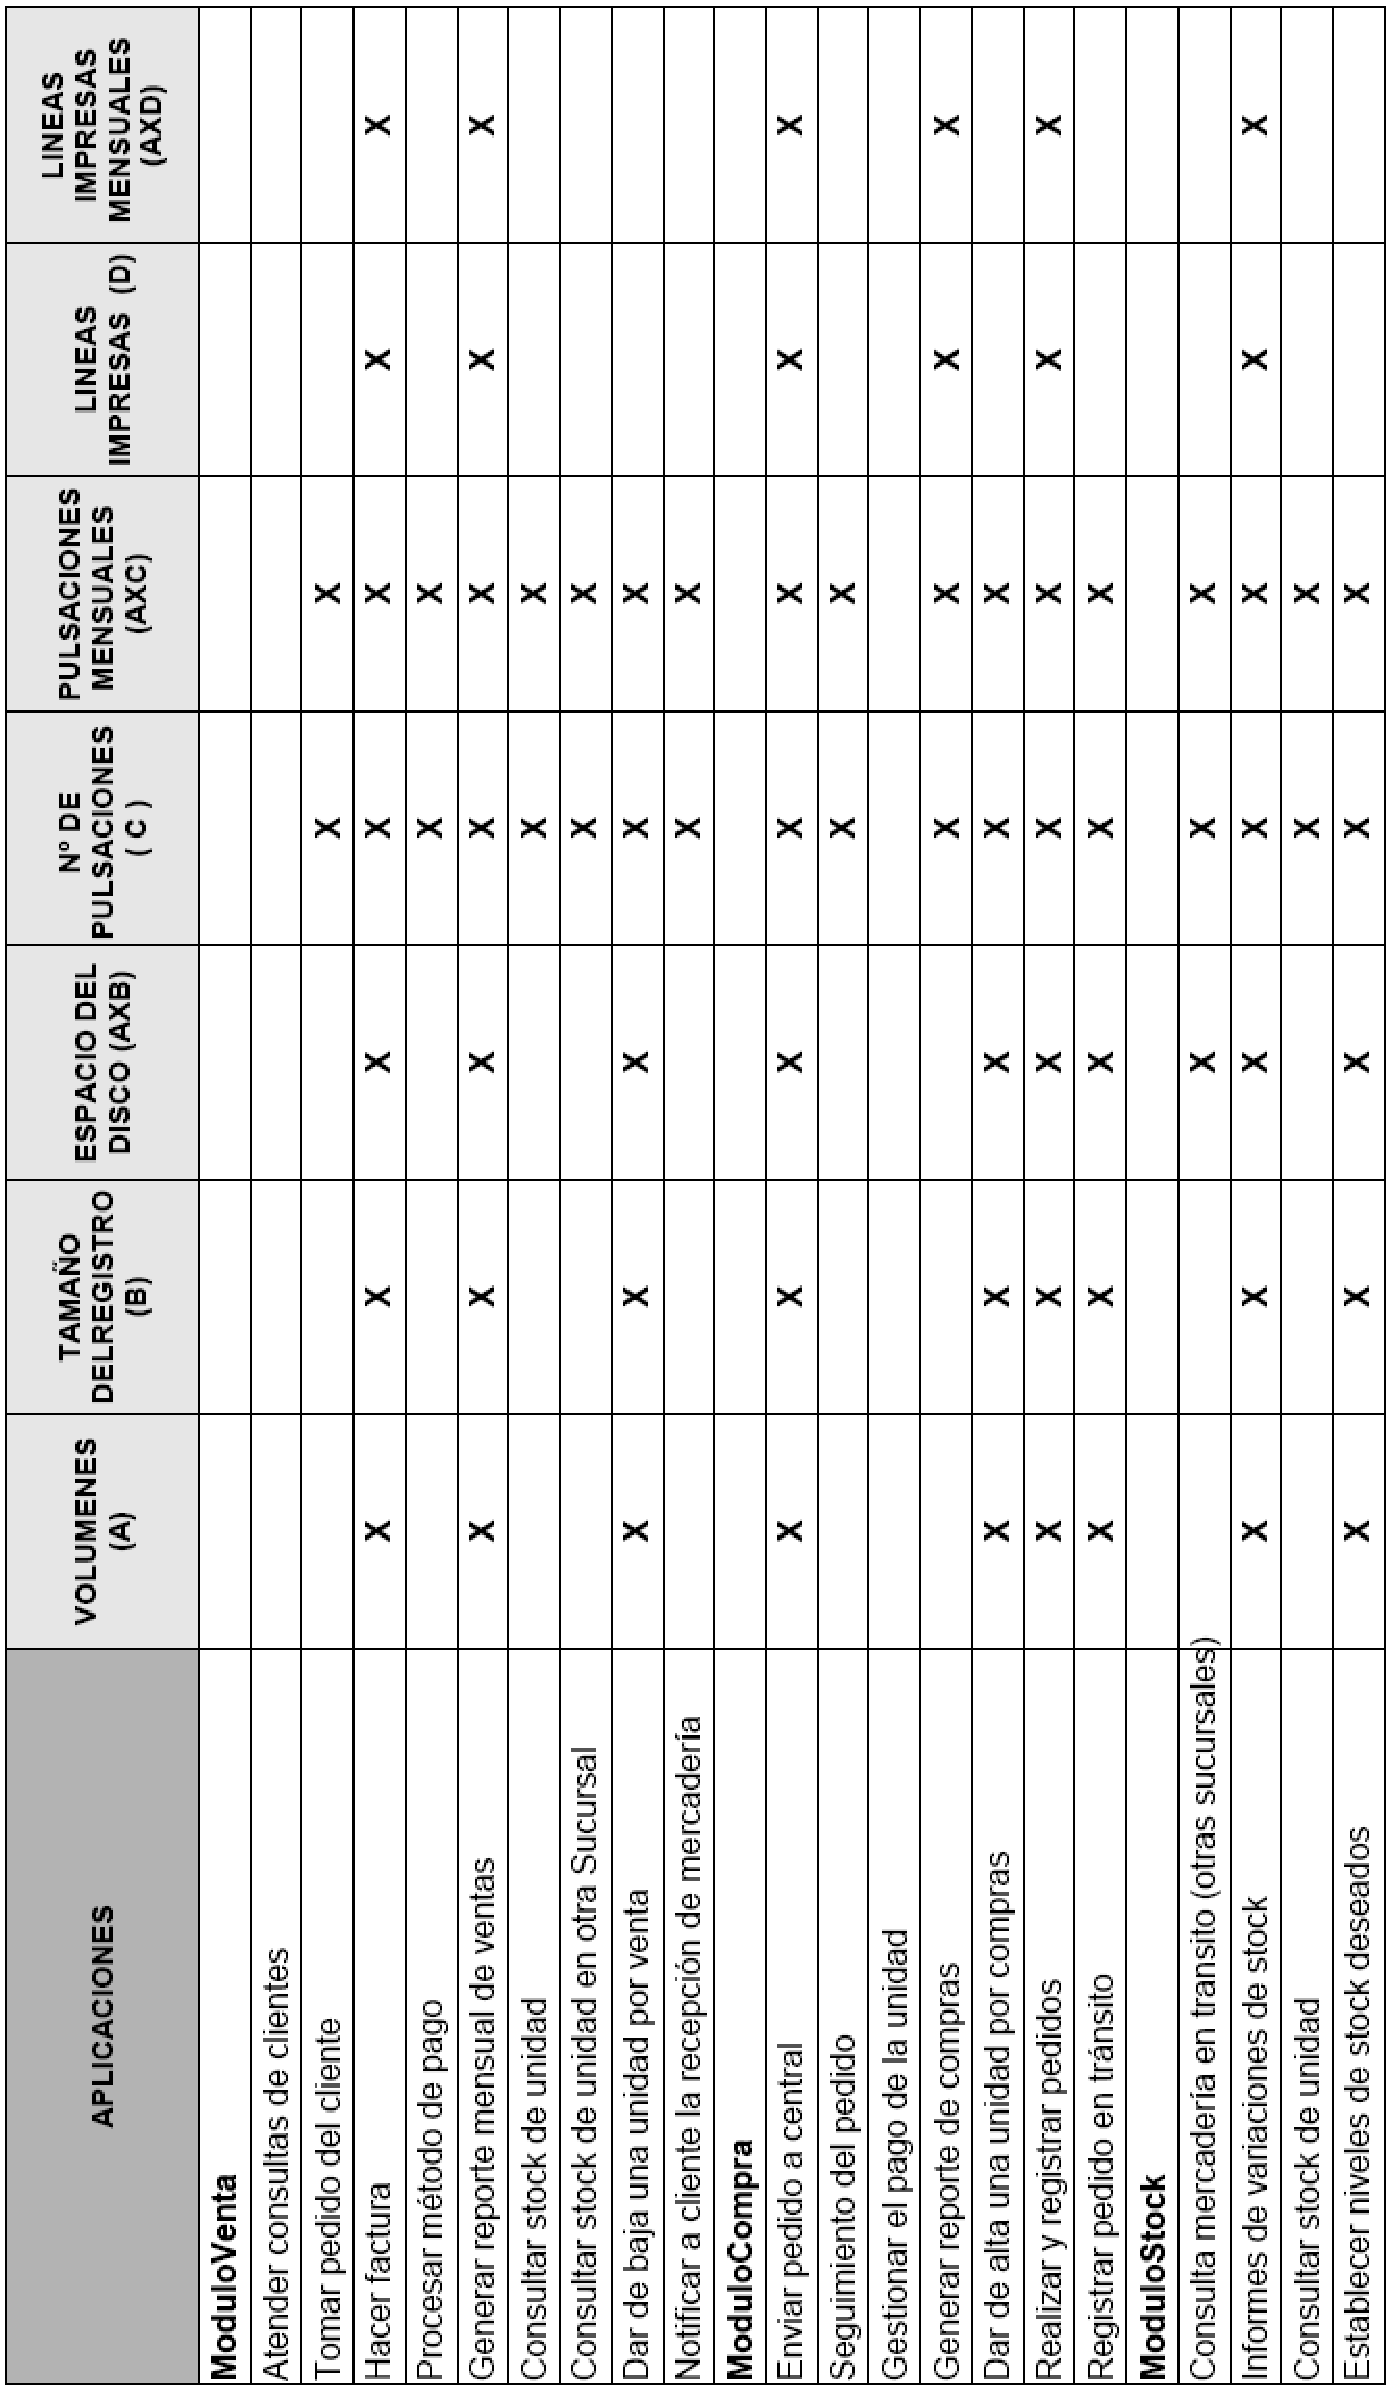
\includegraphics[width=450px]{fase2/volumenes_datos/volumenes_de_datos.pdf}
\end{figure}

\clearpage

\addtolength{\oddsidemargin}{55pt}
\addtolength{\evensidemargin}{70pt}
\addtolength{\topmargin}{90pt}

\subsection{Espacio de almacenamiento:}
\begin{itemize}
  \item \textbf{Espacio de disco requerido para datos:}
  \item \textbf{Espacio requerido para programas:}
  \item \textbf{Total:}
  \item \textbf{Multiplicado por dos (x2):}
  \item \textbf{Espacio de disco requerido para software de base:}
  \item \textbf{Total:}
\end{itemize}

\subsection{Cantidad de puestos para carga de datos:}
\begin{itemize}
  \item \textbf{Cantidad total de pulsaciones mensuales:}
  \item \textbf{Dividido por 22 (días hábiles por mes):}
  \item \textbf{Dividido por 5000 (cantidad de pulsaciones/hora):}
  \item \textbf{Dividido por 6 u 8 (cantidad de hs trabajadas):}
\end{itemize}

\subsection{Cantidad de impresoras de matriz:}
\begin{itemize}
  \item \textbf{Cantidad total de lineas impresas mensuales:}
  \item \textbf{Dividido por 22 (días hábiles por mes):}
  \item \textbf{Dividido por el número de horas diarias (6 u 8):}
  \item \textbf{Dividido por 60:}
\end{itemize}

